\documentclass[tikz,border=2pt]{standalone}
\usepackage{tikz}
\usetikzlibrary{arrows,positioning,shapes}
\begin{document}
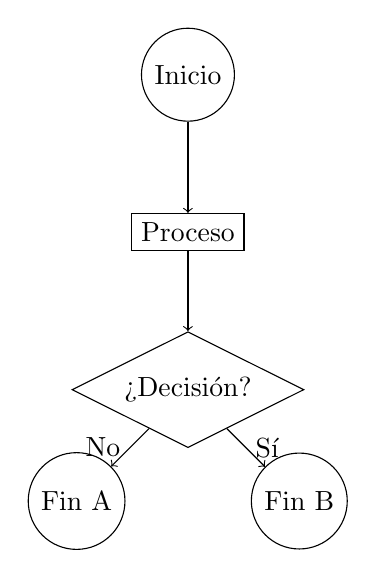
\begin{tikzpicture}[node distance=2cm]
\node (start) [circle, draw] {Inicio};
\node (process) [rectangle, draw, below of=start] {Proceso};
\node (decision) [diamond, draw, aspect=2, below of=process] {¿Decisión?};
\node (end1) [circle, draw, below left of=decision] {Fin A};
\node (end2) [circle, draw, below right of=decision] {Fin B};

\draw[->] (start) -- (process);
\draw[->] (process) -- (decision);
\draw[->] (decision) -- node[left] {No} (end1);
\draw[->] (decision) -- node[right] {Sí} (end2);
\end{tikzpicture}
\end{document}
